\documentclass[12pt]{article}
\usepackage[utf8]{inputenc}
\usepackage[russian]{babel}
\usepackage{amsmath, amssymb}
\usepackage{graphicx}
\usepackage{geometry}
\usepackage{indentfirst}
\usepackage{cite}
\usepackage{hyperref}
\usepackage{csvsimple}
\usepackage{booktabs}   % Для красивых линий (опционально)
\usepackage{caption}
\usepackage{geometry}
\usepackage{etoolbox}
\usepackage{csvsimple}
\usepackage{caption}
\usepackage{float}
\geometry{margin=2cm}
\geometry{a4paper, margin=2.5cm}

\begin{document}

\pagenumbering{gobble}
\begin{titlepage}
    \centering
    \textbf{Московский государственный университет имени М.В. Ломоносова\\
    Филиал в городе Ташенте\\
    Механико-математический факультет\\
    Кафедра Математической теории интеллектуальных систем\\}
    \vfill
    \textbf{\Large{Курсовая работа}}\\
    \vspace{0.5cm}
    по направлению «Прикладная математика и информатика»\\
    на тему: \\
    \vspace{0.5cm}
    \textbf{\Large{Автоматная модель психологического взаимодействия}}\\
    \vfill
    \begin{flushright}
        \textbf{Подготовил:} студент третьего курса ПМиИ\\ Таджиев Георгий Тимурович\\
        \textbf{Научный руководитель:} старший научный сотрудник\\ Волков Николай Юрьевич\\
    \end{flushright}
    \vfill
    Ташкент — 2025
\end{titlepage}
\pagenumbering{arabic}
\clearpage

\begin{abstract}
В данной работе рассматривается автоматная модель психологического взаимодействия между агентами, обладающими эмоциональными состояниями и реляционными функциями. Агенты способны принимать решения о взаимодействиях на основе комплексной оценки отношений и эмоциональных реакций. Реализация выполнена на Python с сохранением результатов в формат CSV для последующего анализа. Исследуется влияние эмоциональной чувствительности и динамики отношений на поведение агентов в обществе.
\end{abstract}

\tableofcontents
\clearpage

\section{Введение}

Моделирование сложных социальных систем с помощью многоагентных симуляций становится важным инструментом для изучения динамики взаимодействий между индивидами. В частности, учет эмоциональных состояний и реляционных функций позволяет более точно описывать процессы принятия решений и формирования отношений в обществе.

Современные исследования в области межагентных систем требуют междисциплинарного подхода, где психология, информатика и социология взаимодействуют для создания более реалистичных моделей. Психологические теории помогают понять эмоциональные и когнитивные механизмы агентов, информатика обеспечивает алгоритмическую реализацию и обработку данных, а социология предлагает концептуальные рамки для анализа социальных структур и динамики. Такой синтез знаний позволяет не только создавать более точные симуляции, но и использовать их для прогнозирования и управления социальными процессами.

Особенно значимым здесь является подход Пикар к аффективным вычислениям [3], подчеркивающий важность учета эмоций при проектировании интеллектуальных систем.

Применение автоматной модели психологического взаимодействия имеет значение в различных областях: от социологии и психологии до информационных технологий и проектирования искусственного интеллекта. Особенно актуальны такие симуляции в условиях, когда прямое экспериментальное изучение человеческих обществ затруднено или неэтично.

В данной работе предлагается автоматная модель психологического взаимодействия агентов, обладающих набором эмоциональных параметров и реляционных функций, которые описывают их социальные и психологические связи. Реляционные функции — это числовые показатели, отражающие качество и характер отношений между агентами. В частности, в модели используются следующие функции:

\begin{itemize}
    \item \textbf{Выгода (utility)} — степень полезности или выгоды, которую агент получает от взаимодействия с другим агентом;
    \item \textbf{Симпатия (affinity)} — эмоциональная положительность или склонность к другому агенту, отражающая чувство доверия и расположения;
    \item \textbf{Доверие (trust)} — уверенность агента в том, что другой агент будет действовать предсказуемо и доброжелательно в будущем взаимодействии;
    \item \textbf{Значимость частоты контактов (responsiveness)} — показатель того, насколько часто и активно агент стремится поддерживать и развивать отношения с другими.
\end{itemize}

Каждый из этих функций принимает значения из ограниченного диапазона \([-10, 10]\), то есть
\[
U_{ij}(t),\; A_{ij}(t),\; T_{ij}(t) \in \mathbb{E}_{21},
\]
а также
\[
R_{ij}(t, U_{ij}(t), A_{ij}(t), T_{ij}(t), \sigma_{i,j}(t))\in \mathbb{E}_{21},
\]
где \(\mathbb{E}_{21} = \{-10, -9, \dots, 10\}\) — множество возможных значений реляционных функций. \(\sigma_{i,j}(t)\) - переменная, описывающая результат взаимодействий \(i\) и \(j\) агентов, к описанию которой мы вернемся позже. 

В модели учитывается, что некоторые психологические качества агентов, такие как базовый архетип и чувствительность, считаются постоянными на протяжении симуляции.
При этом эмоциональные состояния и реляционные функции динамически меняются под воздействием взаимодействий и внешних факторов, влияя на решения агентов и структуру социального сообщества.
Таким образом, модель предоставляет инструмент для изучения комплексных социальных процессов, где эмоции и отношения взаимно влияют друг на друга.
Это позволяет исследовать механизмы устойчивости и изменения социальных связей.

Теоретической основой данной модели являются представления из теории автоматов, в частности концепции автоматных коллективов. Агенты в рассматриваемой модели можно интерпретировать как дискретные автоматы, переходы которых зависят от входных состояний и реляционных параметров. Такой подход согласуется с идеями, изложенными в [1], а также с моделью автоматного взаимодействия, представленной Волковым Н. Ю. в работе [2].


\section{Формальная постановка задачи}


Рассмотрим множество агентов \( \mathcal{K} = \{\mathcal{A}_1, \mathcal{A}_2, \ldots, \mathcal{A}_n \} \), каждый из которых характеризуется вектором эмоциональных состояний \(E_i  \in \mathbb{E}_7^m\), где \(m=7\) — количество осей эмоций.

\subsection*{Постановка задачи моделирования эмоций}

В центре данной работы лежит задача моделирования эмоциональных состояний агентов в социальной среде. Для этого каждому агенту присваивается вектор эмоциональных состояний

\[
E_i = (e_{1}, e_{2}, \ldots, e_{7}) \in \mathbb{E}_7^7,
\]

где \( \mathbb{E}_7 = [-3, 3] \subset \mathbb{Z} \) — допустимый числовой диапазон для каждой из семи независимых осей эмоций, отражающих различные психологические аспекты. Значения компоненты \( e_{ij} \) интерпретируются как интенсивность эмоциональной реакции по соответствующей оси.

В данной модели рассматриваются следующие эмоциональные оси:

\begin{itemize}
    \item Радость — Печаль
    \item Страх — Спокойствие
    \item Гнев — Смирение
    \item Отвращение — Принятие
    \item Удивление — Привычка
    \item Стыд — Уверенность
    \item Открытость — Отчуждение
\end{itemize}

\subsection*{Формализация структуры агента}

Каждый агент \( \mathcal{A}_i \in \mathcal{K} \) в модели представляет собой дискретный автомат, обладающий следующими параметрами:

\begin{itemize}
    \item \textbf{Эмоциональное состояние} \( E_i(t) \in \mathbb{E}_7 \) — вектор значений по 7 независимым осям эмоций;
    \item \textbf{Реляционные функции}
    \[
    U_{ij}(t) \in \mathbb{E}_{21},\quad
    A_{ij}(t)\in \mathbb{E}_{21},\quad
    T_{ij}(t)\in \mathbb{E}_{21},\quad
    R_{ij}(t, U_{ij}(t), A_{ij}(t), T_{ij}(t), \sigma_{i,j}(t))\in \mathbb{E}_{21}
    \]
    — состояние отношения агента \( \mathcal{A}_i \) к агенту \( \mathcal{A}_j \);
    \item \textbf{Архетип} — фиксированная поведенческая стратегия, влияющая на эмоциональную реактивность, чувствительность к отказам и выбор типа взаимодействия;
    \item \textbf{Чувствительность (sensitivity)} — индивидуальный коэффициент, регулирующий скорость изменения эмоций, принимающий значения в интервале \((0, 3]\) и обозначаемый как \( s_i \).\end{itemize}

\paragraph{Логика поведения агента}

Также вводится переменная исхода взаимодействия:
\[
\sigma_{i,j}(t) =
\begin{cases}
    1,  & \text{если взаимодействие состоялось успешно}, \\
    0,  & \text{если взаимодействие не состоялось (отказ)}, \\
    -1, & \text{если взаимодействие состоялось, но неудачно}.
\end{cases}
\]

На каждом шаге симуляции агент:
\begin{enumerate}
    \item Принимает решение о взаимодействии с другим агентом на основе текущих значений функций;
    \item В случае взаимодействия:
    \begin{itemize}
        \item Обновляет своё эмоциональное состояние согласно функции
        \[
        E_i(t+1) = f_i\Bigl(E_i(t),\; s_i\, \bigl\{ U_{ij}(t),\, A_{ij}(t),\, T_{ij}(t),\, R_{ij}(t, U_{ij}(t), A_{ij}(t), T_{ij}(t), \sigma_{i,j}(t)),\, \sigma_{i,j}(t) \bigr\}_{j=1}^n \Bigr),
        \]
        \item Обновляет каждое значение реляционных функции с помощью функций
        \[
        \begin{aligned}
        U_{ij}(t+1) &= g^{(U)}_i(U_{ij}(t), s_i, E_i(t), E_j(t), \sigma_{i,j}(t)), \\
        A_{ij}(t+1) &= g^{(A)}_i(A_{ij}(t), s_i, E_i(t), E_j(t), \sigma_{i,j}(t)), \\
        T_{ij}(t+1) &= g^{(T)}_i(T_{ij}(t), s_i, E_i(t), E_j(t), \sigma_{i,j}(t)), \\
        R_{ij}\bigl(t+1, U_{ij}(t), A_{ij}(t), T_{ij}(t), \sigma_{i,j}(t)\bigr)
        &= g^{(R)}_i\Bigl(R_{ij}\bigl(t, U_{ij}(t), A_{ij}(t), T_{ij}(t), \sigma_{i,j}(t)\bigr),\, s_i, \\
        &\qquad E_i(t),\, E_j(t),\, \sigma_{i,j}(t)\Bigr).
        \end{aligned}
        \]
    \end{itemize}
\end{enumerate}

Функции \( f_i \) и \( g_i \) зависят от параметров архетипа и чувствительности агента \( s_i \) и определяют его индивидуальный стиль поведения в коллективе.
В частности, они задают скорость и направление изменения значений по каждой координате векторов эмоционального состояния и реляционных функций.
Это означает, что агенты с разными архетипами могут по-разному реагировать на одни и те же ситуации:
например, один агент может резко снижать доверие после неудачного взаимодействия, в то время как другой изменяет свои значения реляционных функций более плавно.
Таким образом, \( f_i \) и \( g_i \) моделируют индивидуальные особенности восприятия и реакции на социальные стимулы.
\paragraph{Интерпретация взаимодействия}

Взаимодействие между агентами моделируется как метафорический \emph{разговор по телефону}, в котором участвуют только двое — инициатор и целевой агент. Остальные агенты не слышат этот разговор и не участвуют в нём напрямую. При этом в один такт времени каждый агент выбирает, с кем он хочет взаимодействовать. Условно обозначим за один такт один день, сами дни определяются дискретно, то есть они всегда равны.

\begin{itemize}
    \item \textbf{Успешное взаимодействие} интерпретируется как продуктивный диалог, в ходе которого агенты смогли договориться и остались довольны. Это приводит к положительным изменениям в значений функций доверия, симпатии и выгоды.
    \item \textbf{Неудачное взаимодействие} — ситуация, в которой контакт состоялся, но не принёс удовлетворения (например, из-за разногласий, ссоры или недопонимания). Это приводит к снижению уровня доверия или симпатии.
    \item \textbf{Отказ от взаимодействия} возникает, когда целевой агент отказывается отвечать на попытку контакта. Это решение принимается на основе его текущих зачени реляционных функций к инициатору (например, если отношение к нему негативное или низкая мотивация к взаимодействию).
\end{itemize}

\paragraph{Будущее развитие модели}

В дальнейших версиях планируется ввести механизм \emph{косвенного влияния}, при котором эмоциональное состояние или взаимодействие между двумя агентами может оказывать слабое влияние и на других агентов, если они находятся "рядом" — например, связаны отношениями в сети или входят в общую подгруппу. Это позволит приблизить модель к более реалистичным социальным сценариям, где информация и эмоции распространяются не только напрямую.

\paragraph{Логика выбора взаимодействия}

\subparagraph{Классификация отношений}

На каждом шаге симуляции агент \( \mathcal{A}_i \) рассматривает всех остальных агентов \( \mathcal{A}_j \) и классифицирует их в одну из трёх категорий:

\begin{itemize}
    \item \textbf{Приоритетные (prioritized)} — агенты, с которыми установлены наилучшие отношения, характеризующиеся высокими значениями функций доверия (\( T_{ij} \)), симпатии (\( A_{ij} \)) и/или выгоды (\( U_{ij} \)). Такие агенты рассматриваются как приоритетные цели для взаимодействия;
    \item \textbf{Опциональные (optional)} — агенты с умеренными или неопределёнными отношениями. Взаимодействие с ними возможно, если нет доступных обязательных партнёров;
    \item \textbf{Избегаемые (avoid)} — агенты, по отношению к которым значения ключевых функций (особенно \( A_{ij} \) и \( T_{ij} \)) ниже определённого порога, указывая на недоверие или антипатию. Такие агенты исключаются из рассмотрения.
\end{itemize}

Разделение осуществляется самим агентом. Он анализирует значения текущих реляционных функций агента \( \mathcal{A}_i \) к другому агенту \( \mathcal{A}_j \) и возвращает категорию отношения. Это позволяет имитировать базовую социальную интуицию: избегать тех, кому не доверяешь, тянуться к симпатичным и действовать рационально.

Для выбора цели взаимодействия агент сначала рассматривает кандидатов из обязательной группы.
Если таких нет — выбирает из опциональной.
Цель определяется по максимальному значению функции приоритета:
\[
\text{priority}(j) = A_{ij} + U_{ij} + \alpha \cdot T_{ij} + \beta \cdot R_{ij},
\]
где:
\begin{itemize}
    \item \(A_{ij}\) — симпатия;
    \item \(U_{ij}\) — выгода;
    \item \(T_{ij}\) — доверие;
    \item \(R_{ij}\) — значимость частоты контактов.
\end{itemize}

Коэффициент \(\alpha\) отражает вклад доверия и задаётся в параметрах симуляции (по умолчанию \(\alpha = 1.5\)).
Параметр \(\beta\) зависит от значения \(R_{ij}\): если \(R_{ij} < -7\), применяется усиленный вклад (\(\beta = 1.5\)), иначе — стандартный (\(\beta = 1\)).

Вероятность отказа от взаимодействия зависит от архетипа агента и значения \(R_{ij}\): при низком \(R_{ij}\) шанс отказа увеличивается, но не достигает 100\% (например, может быть 50\%).

Если партнёр отказался от взаимодействия, взаимодействие не происходит.
В этом случае у обоих агентов снижаются значения функций \(R_{ij}\), \(T_{ij}\), \(A_{ij}\) пропорционально чувствительности \( s_i \).

При каждом состоявшемся взаимодействии (независимо от его результата) функция \(R_{ij}\) увеличивается, что отражает рост значимости регулярного контакта.
В случае успеха также повышаются \(U_{ij}\), \(A_{ij}\), \(T_{ij}\), а при неудаче — понижаются.

Таким образом, модель отражает не только факт взаимодействия, но и его качество и последствия.
Это формирует реалистичную динамику социальных отношений.
\subsection*{Подробное описание эмоциональных осей и их психологического смысла}

В модели используются семь пар противоположных эмоций, каждая из которых соответствует оси в многомерном эмоциональном пространстве агента. Каждая ось отражает отдельный психологический аспект и является независимой от других, что позволяет гибко моделировать сложные эмоциональные состояния.

\begin{itemize}
    \item \textbf{Радость — Печаль:} эта ось отражает уровень общего позитивного или негативного настроения. Радость связана с удовлетворением, счастьем и оптимизмом, тогда как печаль — с утратой, грустью и разочарованием. Эти эмоции влияют на мотивацию и социальную активность агента.
    \item \textbf{Страх — Спокойствие:} отражает степень тревожности и беспокойства. Страх проявляется как реакция на угрозу или неопределённость, а спокойствие — как чувство безопасности и расслабленности. Эта ось влияет на готовность к риску и реакцию на стрессовые ситуации.
    \item \textbf{Гнев — Смирение:} связана с агрессивностью и конфликтностью. Гнев выражает раздражение и готовность к борьбе, а смирение — принятие и подчинение. Эти эмоции регулируют уровень конфликтного поведения и разрешения споров.
    \item \textbf{Отвращение — Принятие:} отражает реакцию на неприятные или нежелательные стимулы. Отвращение вызывает отстранённость и отторжение, а принятие — открытость и толерантность. Эта ось влияет на социальную адаптацию и взаимодействие с новыми или непривычными объектами.
    \item \textbf{Удивление — Привычка:} характеризует восприятие новизны и рутинности. Удивление — это реакция на неожиданные события, стимулирующая любопытство, а привычка — комфорт от стабильности и предсказуемости. Эта ось влияет на открытость к изменениям и обучаемость.
    \item \textbf{Стыд — Уверенность:} связана с самооценкой и социальной нормой. Стыд возникает при нарушении ожиданий и вызывает чувство неловкости, а уверенность — ощущение собственной компетентности и социальной поддержки. Эта ось регулирует социальное поведение и саморегуляцию.
    \item \textbf{Открытость — Отчуждение:} отражает степень близости и эмоциональной связи с другими. Открытость характеризуется привязанностью и эмпатией, а отчуждение — отстранённостью и изоляцией. Эта ось определяет качество межличностных отношений и степень социальной интеграции.
\end{itemize}

\paragraph{Математическая модель эмоций}

Эмоции каждого агента моделируются в виде вектора

%
\[
E_i = (e_{i1}, e_{i2}, \ldots, e_{i7}) \in\mathbb{E}_7^7,
\]

где каждое значение \( e_{ij} \) — числовая характеристика интенсивности эмоции по соответствующей оси. Значения варьируются от -3 (максимально отрицательный полюс) до +3 (максимально положительный).

\paragraph{Постоянные и переменные параметры}

В модели:

\begin{itemize}
    \item \textbf{Постоянные параметры:} архетип агента и чувствительность к изменениям  \( s_i \) (sensitivity), которые определяют базовую психологическую структуру и степень восприимчивости к эмоциональным и социальным воздействиям.
    \item \textbf{Переменные параметры:} вектор эмоциональных состояний \(E_i\) и реляционные функции (\(U_{ij}\) выгода, \(A_{ij}\) симпатия, \(T_{ij}\) доверие, \(R_{ij}\) значимость контактов), которые динамически изменяются в ходе взаимодействий и под влиянием внешних факторов.
\end{itemize}

Такой подход обеспечивает реалистичное моделирование эмоциональной динамики, позволяя агентам адаптироваться к социальному окружению, сохраняя при этом индивидуальные психологические характеристики.

\paragraph{Независимость осей эмоций}

Мы исходим из предположения, что каждая ось эмоций является статистически независимой, то есть интенсивность одной эмоции не предопределяет значения другой. Это позволяет модели гибко сочетать различные эмоциональные состояния и отражать сложность человеческой психики.

Каждая ось представляет собой целочисленный отрезок от отрицательного к положительному полюсу, и значение \( e_{ij} \) характеризует интенсивность эмоции по соответствующей оси для агента \( \mathcal{A}_i \).

Правила обновления эмоциональных состояний основаны на взаимодействиях агентов и влиянии значений реляционных функций. Изменения могут быть как в сторону усиления положительных эмоций, так и усиления негативных, что отражает сложную динамику эмоциональных реакций.

Такая постановка задачи позволяет формализовать эмоциональные состояния в многомерном пространстве, что является основой для анализа и симуляции психологического взаимодействия в социальной группе.

\bigskip

Каждое взаимодействие между агентами \( \mathcal{A}_i \) и \( \mathcal{A}_j \) определяется набором реляционных функций:

\[
U_{ij}, A_{ij}, T_{ij}, R_{ij} 
\]

где:

\begin{itemize}
    \item \( U_{ij} \) — выгода агента \( \mathcal{A}_i \) от взаимодействия с \( \mathcal{A}_j \). Отражает степень полезности или результата, который получает агент, то есть насколько выгодно или приятно для него это взаимодействие с точки зрения личных интересов.
    \item \( A_{ij} \) — симпатия агента \( \mathcal{A}_i \) к \( \mathcal{A}_j \). Это эмоциональное расположение или положительное отношение, которое не обязательно связано с рациональной оценкой поведения партнёра.
    \item \( T_{ij} \) — доверие агента \( \mathcal{A}_i \) к \( \mathcal{A}_j \). Это ожидание, что партнёр будет вести себя предсказуемо и доброжелательно, обеспечивая стабильность взаимодействия.
    \item \( R_{ij} \) — значимость для агента \( \mathcal{A}_i \) частоты контактов с \( \mathcal{A}_j \). Отражает насколько важна регулярность и частота взаимодействий для поддержания и развития отношений, показывая, как частота общения влияет на прочность связи.
\end{itemize}

В отличие от прочих функций, значение \( \sigma_{i,j}(t) \) определяется детерминированно для \(0\) (отказ) и случайно для исходов \(\pm 1\) в рамках заданной вероятностной модели.

Важно понимать, что эти параметры описывают разные аспекты психологических отношений и в нашей модели считаются независимыми. 


Мы исходим из того, что эти психологические параметры являются независимыми, и значение каждой функции не предопределяет значения других. Это означает, что любые сочетания значений реляционных функций возможны и рассматриваются как равновероятные в модели.


Подход к формализации доверия в данной работе во многом опирается на когнитивную модель доверия, разработанную Кастельфранчи и Фальконе~[4]. Согласно этой модели, доверие рассматривается как сложный когнитивный процесс, включающий оценку надежности и доброжелательности другого субъекта на основе имеющейся информации и прошлых взаимодействий.

Основные компоненты когнитивной модели доверия включают:

\begin{itemize}
    \item \textbf{Оценка компетентности и надежности}: агент оценивает, насколько другой агент способен выполнить ожидаемые действия и придерживаться договоренностей.
    \item \textbf{Оценка намерений}: помимо способности, оценивается доброжелательность и намерения партнёра, то есть готовность действовать в интересах доверяющего.
    \item \textbf{Ожидания от поведения}: на основе предыдущего опыта формируются ожидания о будущем поведении партнёра, которые влияют на решение о взаимодействии.
    \item \textbf{Контекстуальная зависимость}: доверие может меняться в зависимости от ситуации, целей и окружения, в котором происходит взаимодействие.
\end{itemize}

В модели Кастельфранчи и Фальконе доверие не является статичной характеристикой, а динамически обновляется по мере получения новой информации и взаимодействия с партнёром. Это согласуется с подходом нашей модели, где доверие \( T_{ij} \) между агентами изменяется во времени в зависимости от успешности и характера их взаимодействий.

Таким образом, когнитивная модель доверия помогает формализовать и обосновать динамическое поведение функций доверия в нашей автоматной модели психологического взаимодействия, обеспечивая более глубокое понимание механизмов социальных отношений и принятия решений в мультиагентных системах.



\subsection*{Роль параметров устойчивости отношений и функция разрыва связи}

Важным аспектом модели является учет параметров устойчивости (стабильности) отношений между агентами. Эти параметры отражают способность отношений сохраняться или изменяться под воздействием внешних и внутренних факторов. Введена функция "разрыва" связи, которая активируется при достижении определенного порога негативных изменений в значениях функций, особенно в доверии и симпатии. Такая функция моделирует ситуацию, когда связь между агентами прекращается, что влияет на структуру сети взаимодействий и дальнейшее поведение агентов.

Цель модели — описать динамику изменения эмоциональных состояний \(E_i\) и функций \(U_{ij}, A_{ij}, T_{ij}, R_{ij} \) под воздействием взаимодействий, а также влияние появления новых агентов в системе.



Вместо этого изменения зависят непосредственно от текущих значений эмоций и функций, а учет долгосрочной истории взаимодействий планируется добавить в будущих версиях модели.




В данной модели функции \( f_i \) и \( g_i \) напрямую зависят от архетипа агента, который представляет собой обобщённый тип психологического поведения. Архетип определяет типичные эмоциональные реакции и особенности восприятия отношений. В частности, в модели используются следующие архетипы:


\begin{itemize}
    \item \textbf{Erudition (Мудрец)} — хладнокровный, избегает крайностей, эмоционально стабилен, ценит знание и логику. Реже инициирует эмоциональные реакции, проявляет рациональность в выборе взаимодействий.
    \item \textbf{Enigmata (Бунтарь)} — импульсивный и склонный к конфликту архетип, с повышенной вероятностью отказов от взаимодействий. Часто действует наперекор ожиданиям, провоцируя эмоциональные всплески.
    \item \textbf{Harmony (Гармоничный)} — стремится к балансу и согласию. Склонен принимать предложения о взаимодействии, повышенно чувствителен к симпатии и доверию.
    \item \textbf{Hunt (Воин)} — решительный и смелый, архетип с низкой чувствительностью к страху и отвращению. Быстро реагирует на угрозы, активно участвует в конфликтах.
    \item \textbf{Elation (Трикстер)} — непредсказуем, легко переключается между эмоциями. Взаимодействует спонтанно, часто влияет на эмоциональные состояния других.
    \item \textbf{Preservation (Страж)} — охранительный архетип, заботится о других, склонен к устойчивым связям. Повышенно чувствителен к чувству вины и долга.
    \item \textbf{Nihility (Тайна)} — сосредоточен на распаде, сомнении, исчезновении. Склонен разрушать устойчивые связи, вносит хаос в отношения.
    \item \textbf{Trailblaze (Путеводитель)} — уравновешен и открыт к новому, ищет смысл во взаимодействиях, инициирует связи на основе интеллектуальной и моральной оценки.
    \item \textbf{Remembrance (Память)} — ориентирован на прошлое, устойчив к эмоциональным колебаниям, склонен к рефлексии и сохранению долгосрочных связей.
\end{itemize}

Каждый из этих архетипов задаёт не только характер поведения агента, но и параметры функций \( f_i \) и \( g_i \), определяя стиль реагирования на взаимодействия, вероятность отказа и эмоциональную реактивность.

Архетип влияет на параметры функций \( f_i \) и \( g_i \), определяя, например, насколько сильна реакция на отказ или насколько быстро изменяется доверие. Таким образом, архетип является ключевым элементом, задающим индивидуальное поведение агента в рамках универсальных правил модели.
\bigskip

%
\[
E_i(t+1) = f\Bigl(E_i(t),\; \bigl\{ U_{ij}(t),\, A_{ij}(t),\, T_{ij}(t),\, R_{ij}(t, U_{ij}(t), A_{ij}(t), T_{ij}(t), \sigma_{i,j}(t)) \bigr\}_{j=1}^n \Bigr),
\]

\[
\begin{aligned}
U_{ij}(t+1) &= g^{(U)}_i\big(U_{ij}(t), s_i, E_i(t), E_j(t), \sigma_{i,j}(t)\big), \\
A_{ij}(t+1) &= g^{(A)}_i\big(A_{ij}(t), s_i, E_i(t), E_j(t), \sigma_{i,j}(t)\big), \\
T_{ij}(t+1) &= g^{(T)}_i\big(T_{ij}(t), s_i, E_i(t), E_j(t), \sigma_{i,j}(t)\big), \\
R_{ij}(t+1, U_{ij}(t), A_{ij}(t), T_{ij}(t), \sigma_{i,j}(t)) &= g^{(R)}_i\big(R_{ij}(t, U_{ij}(t), A_{ij}(t), T_{ij}(t), \sigma_{i,j}(t)), s_i, E_i(t), E_j(t), \sigma_{i,j}(t)\big),
\end{aligned}
\]

где каждая функция \( g^{(\cdot)}_i \) представляет собой компоненту индивидуальной стратегии агента \( \mathcal{A}_i \) по обновлению соответствующей реляционной функции.

В дальнейшем предусмотрено расширение модели с включением формализованной истории взаимодействий для более точного моделирования динамики отношений.

\subsection*{Определение коллектива}

Под \textbf{коллективом} в данной модели понимается множество агентов \( \mathcal{K} = \{\mathcal{A}_1, \mathcal{A}_2, \ldots, \mathcal{A}_n \} \), находящихся в общем социальном пространстве и способных вступать во взаимодействия друг с другом. Коллектив обладает следующими характеристиками:

\begin{itemize}
    \item Каждый агент обладает индивидуальными параметрами: вектором эмоций \( E_i \), архетипом, чувствительностью \( s_i \) и реляционными функциями \( \{ U_{ij}, A_{ij}, T_{ij}, R_{ij} \} \) по отношению к каждому другому агенту;
    \item Взаимодействие между агентами осуществляется на каждом шаге симуляции по правилам, зависящим от их значения реляционных функций и стратегии выбора цели;
    \item Коллектив может дополняться новыми агентами, при этом для каждого устанавливаются начальные значения реляционных функций к уже существующим агентам;
    \item Поведение агентов в коллективе описывается как система взаимосвязанных автоматов, принимающих решения и изменяющих своё состояние во времени.
\end{itemize}

Таким образом, коллектив является динамически изменяющейся системой, в которой моделируется сложное социально-психологическое взаимодействие между индивидуумами.

\section{Структура и реализация модели}

Модель реализована на языке Python с использованием модульного и объектно-ориентированного подхода. Основные компоненты:

\begin{itemize}
    \item \textbf{Класс Agent}: хранит эмоциональное состояние, значения реляционных фунуций к другим агентам, методы для обновления состояний и принятия решений.
    \item \textbf{Класс Collective}: управляет всеми агентами и игроками, координирует их взаимодействия, реакции, обновление отношений и эмоций. Отвечает за симуляцию дня и стратегию принятия решений.
    \item \textbf{Среда Simulation}: управляет временем симуляции, отслеживает дату, запускает процесс взаимодействия и регистрирует историю.
    \item \textbf{Концептуальная основа}: модель базируется на идеях теории автоматов, где каждый агент представлен как дискретный автомат с внутренним состоянием и переходами, зависящими от эмоций и отношений. Подход опирается на принципы агентных систем, отражённые в дорожной карте исследований в области автономных агентов и мультиагентных систем[5]. Основными концептуальными принципами модели являются:
    \begin{itemize}
        \item \textit{Агентная автономия}: каждый агент самостоятельно принимает решения на основе своих эмоциональных состояний и значений реляционных функций.
        \item \textit{Модульность поведения}: поведение агента определяется архетипом и чувствительностью, что позволяет гибко варьировать стратегии реакции.
        \item \textit{Эволюция отношений}: взаимодействия между агентами приводят к обновлению значений функций, что отражает адаптивную природу социальных связей.
        \item \textit{Дискретное время}: симуляция развивается по шагам, на каждом из которых происходит анализ и обновление эмоциональных и социальных состояний.
    \end{itemize}
    \item \textbf{Модуль анализа}: сохраняет результаты в CSV-файлы с информацией о состоянии агентов и значениях реляционных функций на каждом шаге симуляции, а также историю всех взаимодействий.
\end{itemize}

Обновление эмоциональных состояний происходит с учетом текущих значений функций и эмоциональных реакций на взаимодействия. Реляционные функции корректируются в зависимости от успешности взаимодействий и частоты контактов.

Добавление новых агентов осуществляется по заданным правилам, что позволяет исследовать влияние притока новых участников на структуру и динамику общества.

\begin{figure}[h!]
    \centering
    \begin{minipage}[b]{0.45\textwidth}
        \centering
        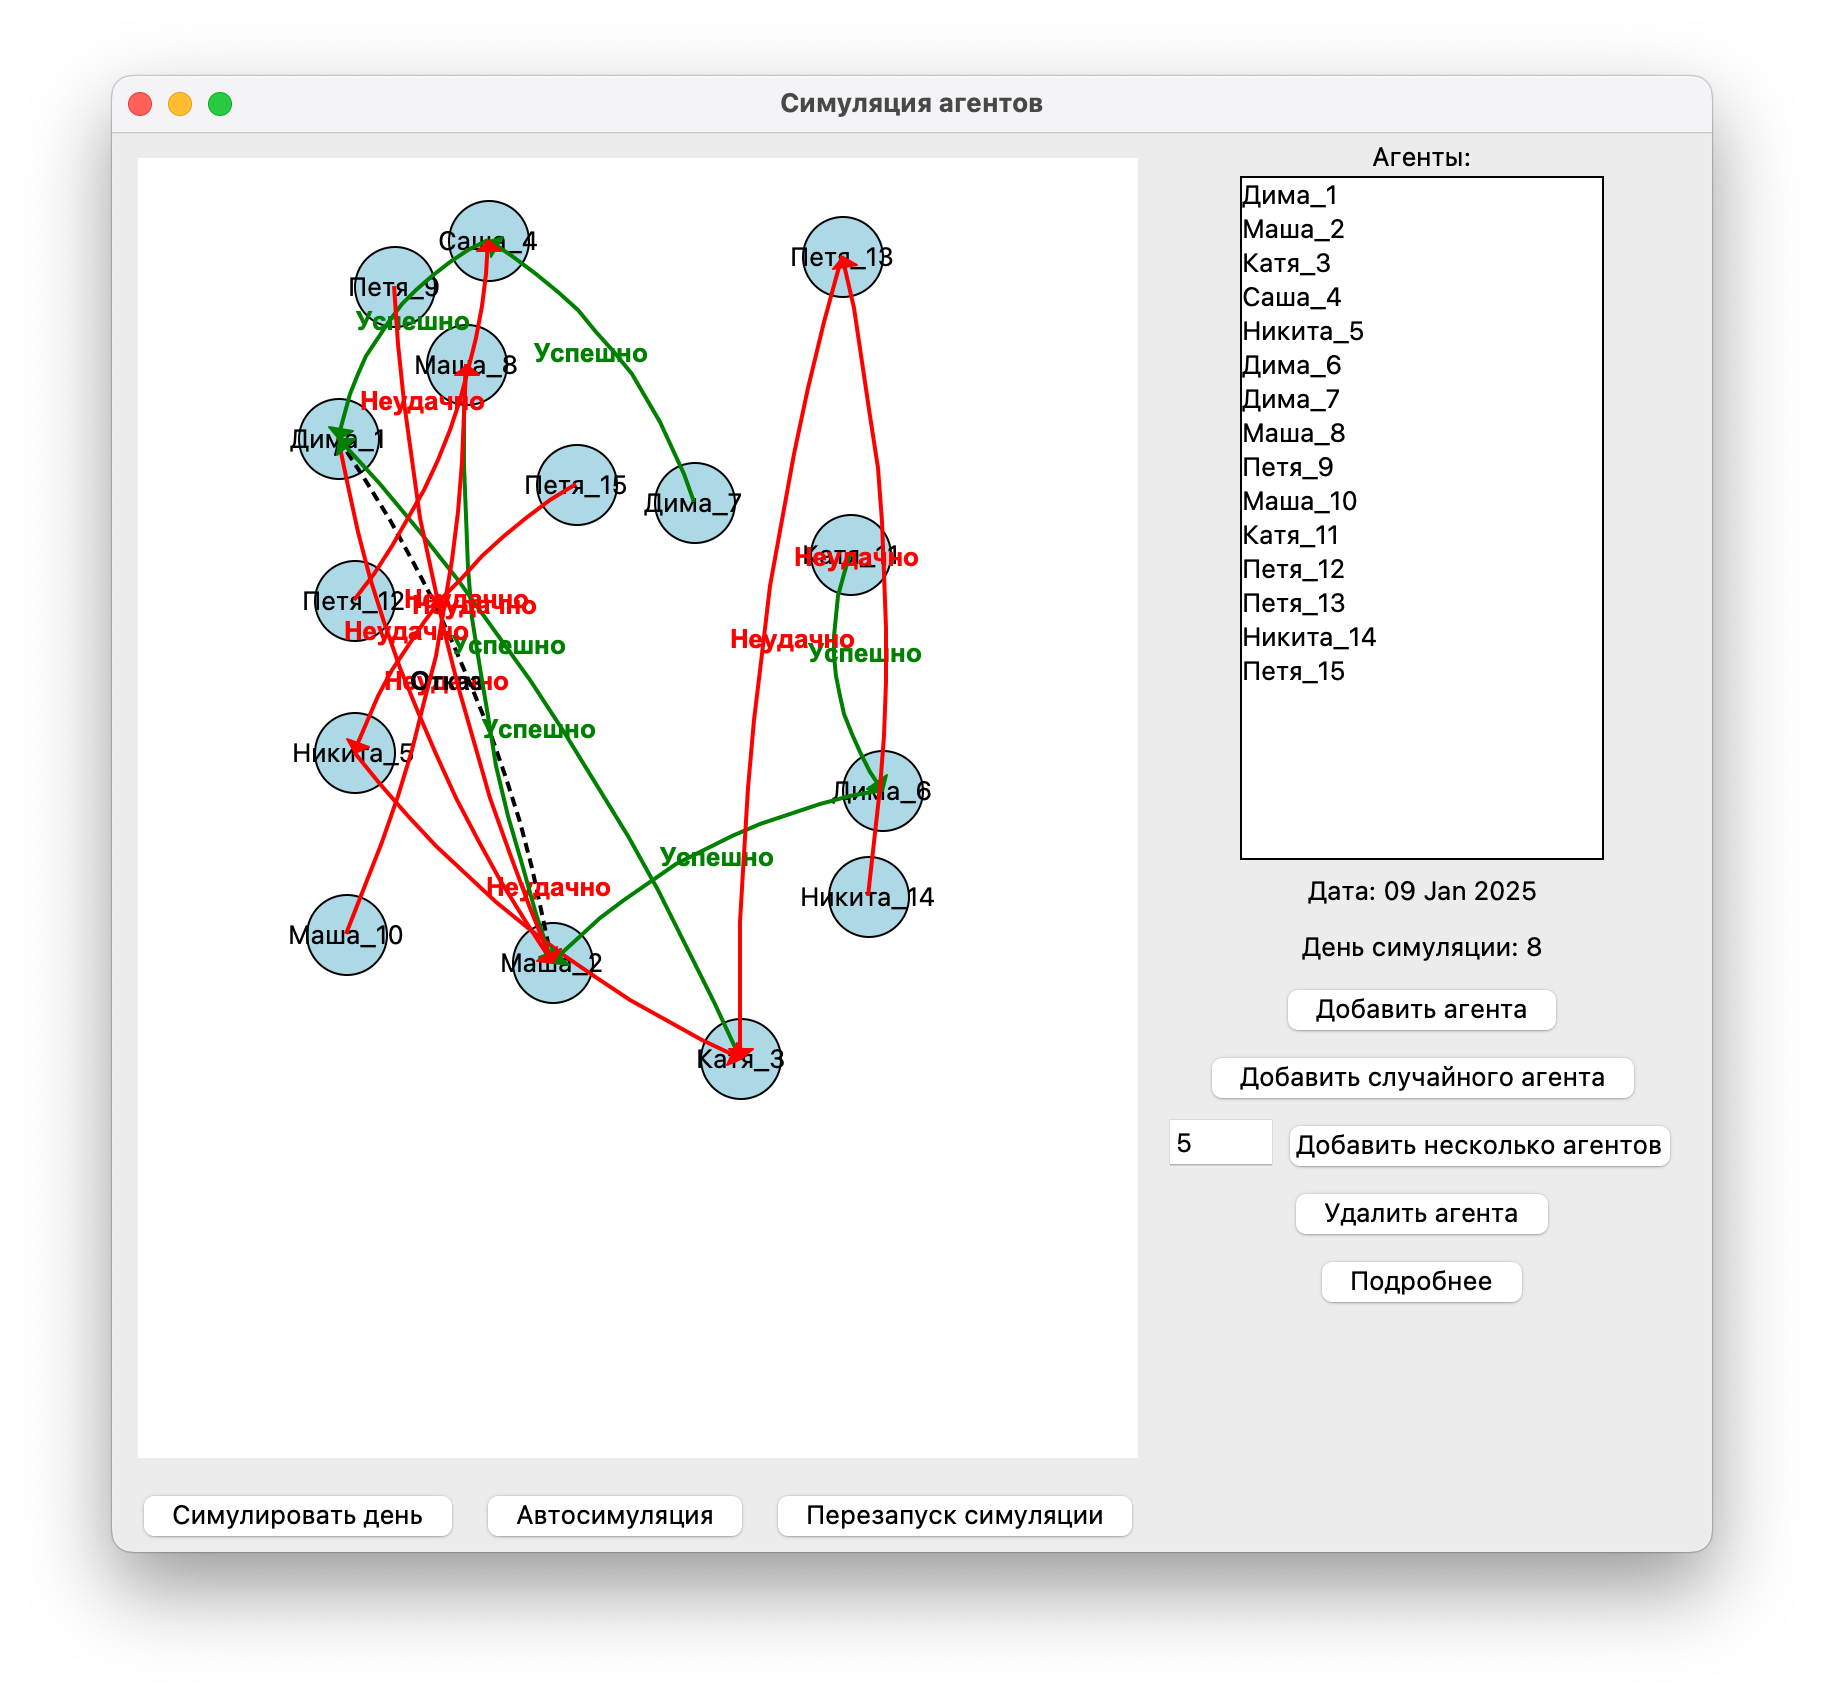
\includegraphics[width=\textwidth]{Снимок экрана 2025-05-23 в 20.28.29.png}
        \caption{Пример взаимодействия агентов на графе в интерфейсе программы}
        \label{fig:interaction-example}
    \end{minipage}
    \hspace{0.05\textwidth}
    \begin{minipage}[b]{0.45\textwidth}
        \centering
        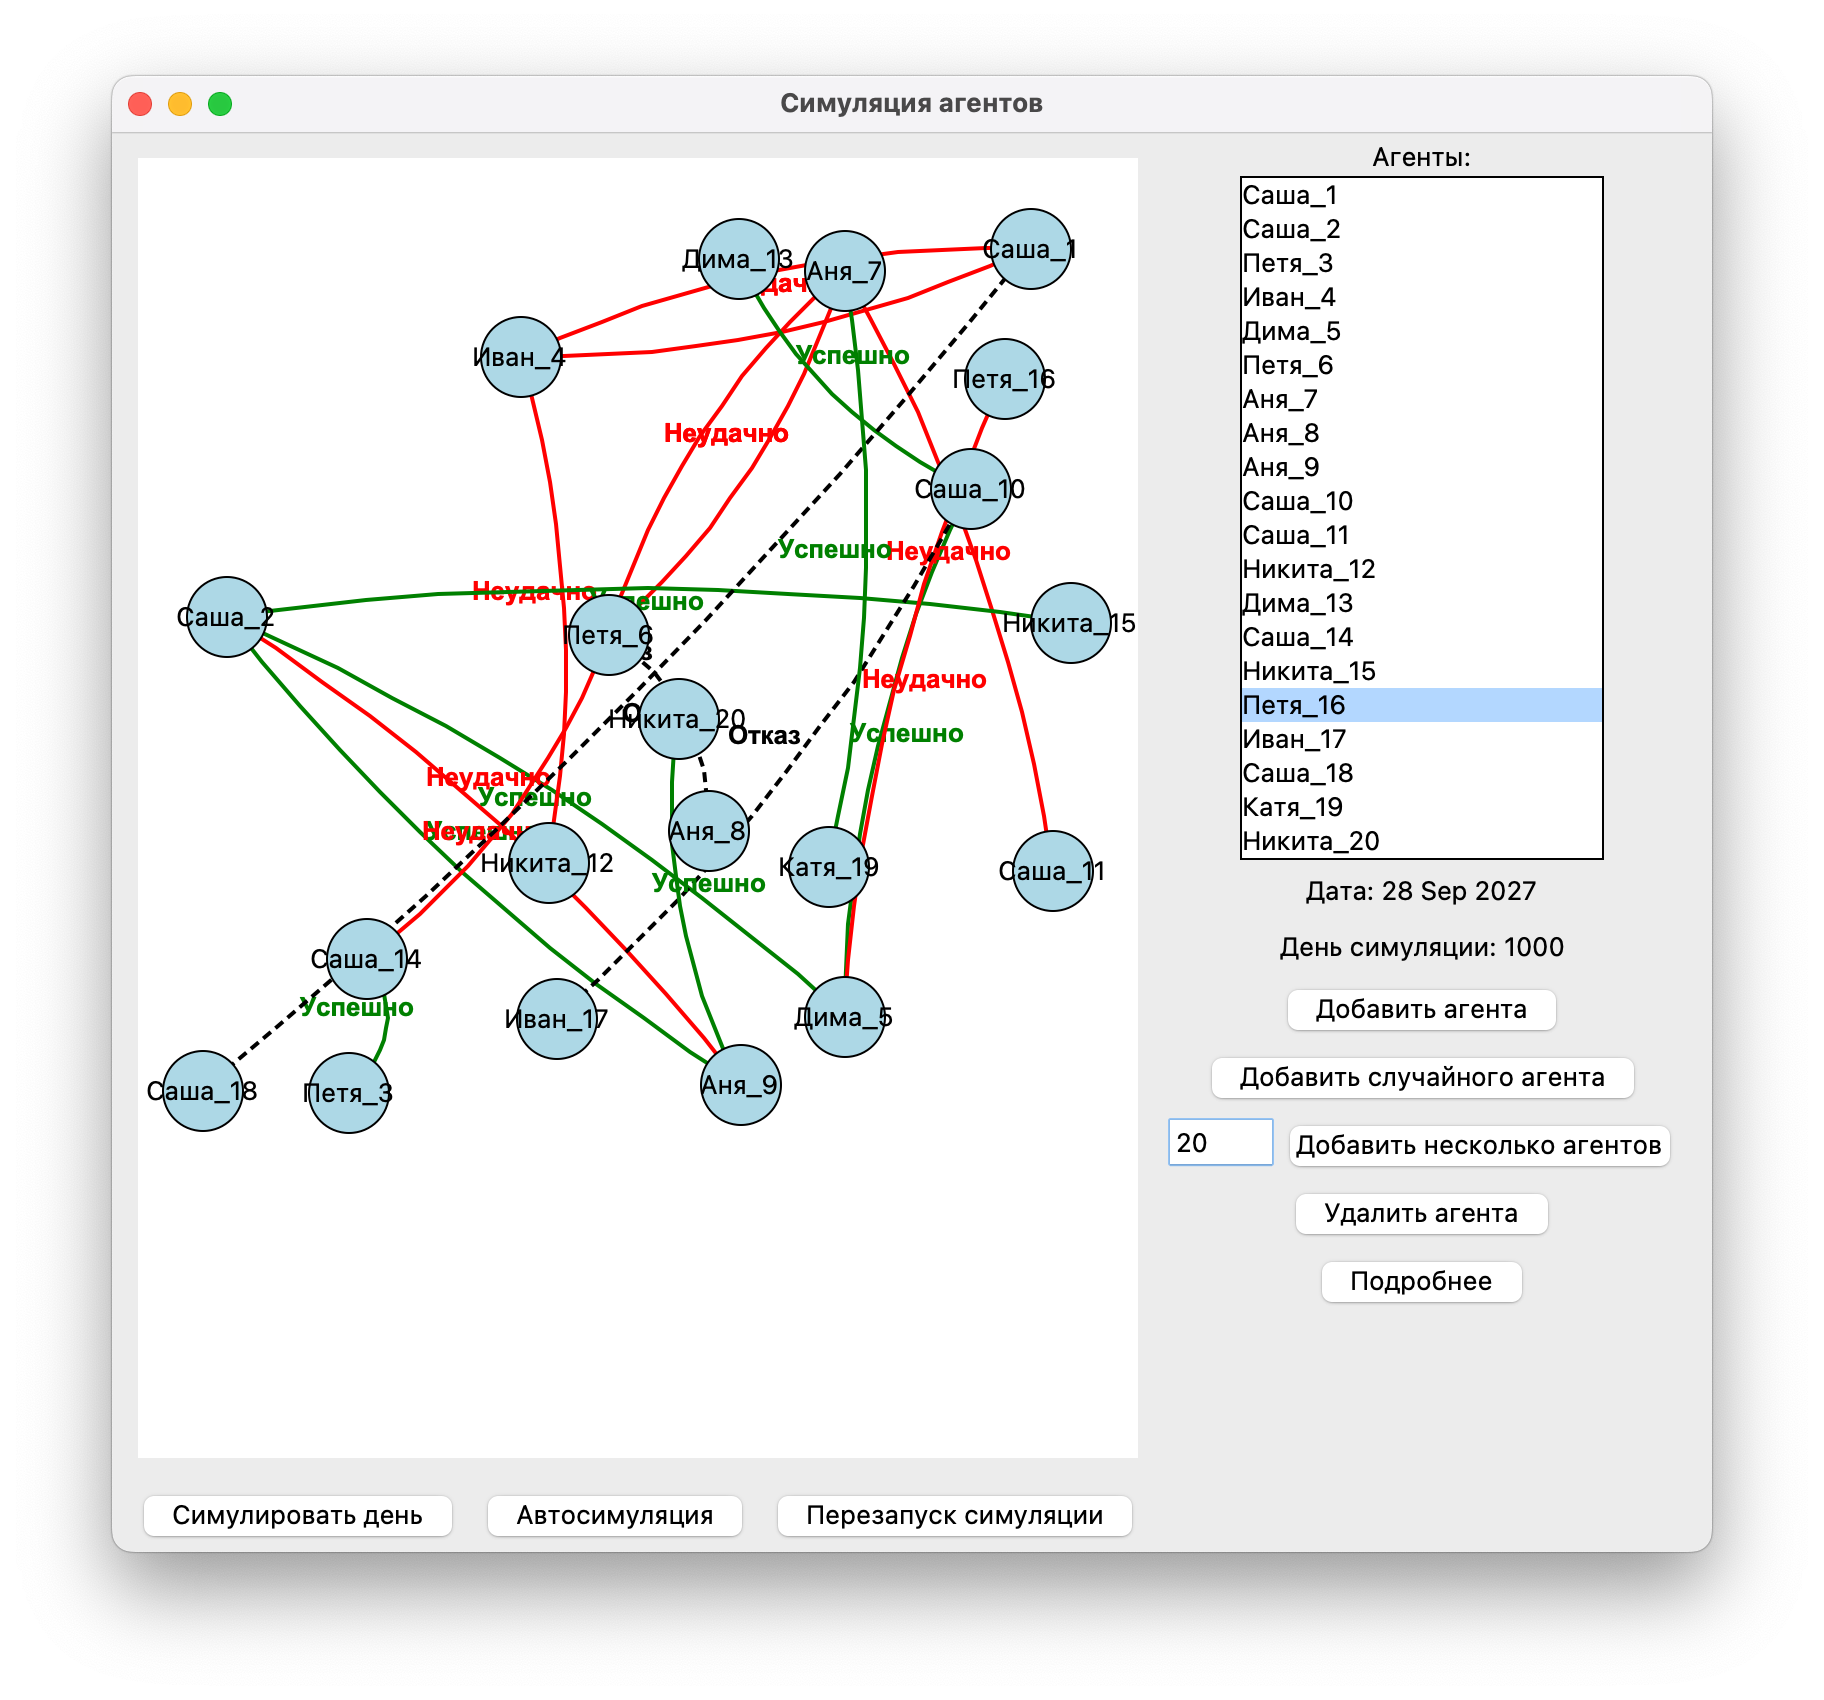
\includegraphics[width=\textwidth]{Снимок экрана 2025-05-23 в 22.50.51.png}
        \caption{Пример взаимодействия агентов на графе на 1000 день}
        \label{fig:interaction-example-1000}
    \end{minipage}
\end{figure}

\section{Результаты симуляции и анализ}

В ходе экспериментов были проведены серии из 50 симуляций длиной по 1000 дней с 20 агентами с различными параметрами чувствительности \( s_i \) агентов и начальной конфигурацией сети взаимодействий. Полученные данные позволили сделать следующие наблюдения:

\begin{itemize}
    \item Повышенная чувствительность агентов к частоте контактов (\(responsiveness\)) способствует формированию устойчивых кластеров с высоким уровнем доверия, симпатии и повторяемости взаимодействий. Это отражается в высоком среднем количестве часто взаимодействующих пар (в среднем 49 из 78.6).
    
    \item Система демонстрирует склонность к самоорганизации: в каждой симуляции образуется в среднем 5 полносвязных групп из трёх и более агентов, что подтверждает появление устойчивых микросообществ.
    
    \item Несмотря на общее стремление к стабильности, сохраняется значительная вариативность: минимальное число взаимодействий между парами всегда остаётся равным 1, тогда как максимумы достигают значений порядка 1980. Это говорит о наличии как сильно вовлечённых, так и изолированных агентов.
    
    \item Введение новых агентов в процессе симуляции приводит к перераспределению значений реляционных функций, а также к изменению эмоционального фона, что может нарушать уже сложившиеся связи и провоцировать перестройку сети.
    
    \item Эмоциональные состояния агентов демонстрируют циклические колебания, отражающие регулярные и отклоняющиеся взаимодействия. Эти циклы коррелируют с пиками и падениями в метриках доверия, выгоды и симпатии.
    
    \item Сохранение результатов симуляций в формате CSV обеспечило прозрачность анализа и позволило провести агрегированный статистический разбор поведения модели, в том числе по числу взаимодействий, структуре пар и формированию групп.
\end{itemize}
% --- Таблица 1: Общие метрики взаимодействий ---
\begin{table}[H]
\centering
\caption{Общие метрики взаимодействий}
{\footnotesize
\begin{tabular}{|c|c|c|c|}
\hline
Номер прогона & Среднее & Максимум & Минимум \\
\hline
\csvreader[
    late after line=\\\hline,
    filter expr={test{\ifnumless{\thecsvinputline}{52}}}
]{summary_stats.csv}{}%
{\csvcoli & \csvcolii & \csvcoliii & \csvcoliv}
\textbf{Среднее} & \textbf{175.14} & \textbf{1371.72} & \textbf{1.0} \\
\hline
\end{tabular}
}
\end{table}
\newpage

Результаты демонстрируют высокий разброс количества взаимодействий между агентами.  
Среднее значение (175.14) указывает на достаточно активную модель, в которой большинство агентов регулярно вступают в контакты.  
Минимальное значение всегда равно 1, что говорит о наличии слабо включённых агентов или непопулярных пар.  
Максимальные значения (до 1983) свидетельствуют о формировании устойчивых коммуникационных пар или цепочек.


\vspace{1em}

% --- Таблица 2: Частота взаимодействий в парах ---
\begin{table}[H]
\centering
\caption{Типы парных взаимодействий}
{\footnotesize
\begin{tabular}{|c|c|c|c|c|}
\hline
Номер прогона & Всего пар & Редко & Иногда & Часто \\
\hline
\csvreader[
    late after line=\\\hline,
    filter expr={test{\ifnumless{\thecsvinputline}{52}}}
]{summary_stats.csv}{}%
{\csvcoli & \csvcolv & \csvcolvi & \csvcolvii & \csvcolviii}
\textbf{Среднее} & \textbf{78.58} & \textbf{20.58} & \textbf{9.0} & \textbf{49.0} \\
\hline
\end{tabular}
}
\end{table}
\newpage

Модель демонстрирует склонность к формированию устойчивых пар: в среднем 49 из 78.6 взаимодействий относятся к категории «часто».  
Это подтверждает, что агенты склонны повторно вступать в одни и те же связи, что характерно для устойчивых социально-эмоциональных структур.  
Категории «редко» и «иногда» встречаются значительно реже, что может свидетельствовать о фильтрации неперспективных связей.


\vspace{1em}

% --- Таблица 3: Группы агентов с полными связями (≥3) ---
\begin{table}[H]
\centering
\caption{Полносвязные группы агентов (3 и более)}
{\footnotesize
\begin{tabular}{|c|c|}
\hline
Номер прогона & Групп ($\geq$3) \\
\hline
\csvreader[
    late after line=\\\hline,
    filter expr={test{\ifnumless{\thecsvinputline}{52}}}
]{summary_stats.csv}{}%
{\csvcoli & \csvcolix}
\textbf{Среднее} & \textbf{5} \\
\hline
\end{tabular}
}
\end{table}

\newpage

Модель способна формировать устойчивые группы из трёх и более агентов, в среднем 5 таких групп на симуляцию.  
Это указывает на склонность системы к самоорганизации и кластеризации — агентов тянет к стабильным микросообществам.  
Чем выше чувствительность к частоте контактов, тем выше вероятность формирования таких ядер.

Приведенные результаты подтверждают важность учета эмоциональных и реляционных факторов при моделировании межагентных взаимодействий.

Анализ поведения агентов показал, что система демонстрирует признаки самоорганизации: возникают устойчивые подструктуры, а отдельные агенты занимают центральные роли в коммуникационной сети. Эти наблюдения могут быть полезны при проектировании социальных платформ, распределённых систем и симуляции кризисных ситуаций.

Таким образом, результаты симуляций подтверждают эффективность предложенной модели и открывают перспективы для дальнейших исследований.

\section{Заключение}

В данной работе была разработана и реализована модель симуляции межагентных взаимодействий, учитывающая эмоциональные состояния и реляционные функции. Модель демонстрирует, что эмоциональная чувствительность и динамика отношений существенно влияют на поведение агентов и структуру общества.

Предложенная модель учитывает постоянные психологические характеристики агентов, такие как архетип и чувствительность, а также динамические изменения эмоциональных состояний и реляционных функций. Это позволяет исследовать сложные механизмы формирования и эволюции социальных отношений в группе, обеспечивая более глубокое понимание межагентных взаимодействий.

Таким образом, выполненная работа создает основу для дальнейших исследований и практических применений в области моделирования социальных систем.

Автор выражает благодарность научному руководителю, старшему научному сотруднику Волкову Николаю Юрьевичу за ценные советы и поддержку в процессе разработки модели.

Также автор благодарит Валентину Владимировну Ушакову за методическую поддержку и вдохновляющие обсуждения, оказавшие влияние на развитие концепции модели.


\clearpage
\section{Список литературы}

\begin{enumerate}
    \item Кудрявцев В. Б., Алешин С. В., Подколзин А. С. Теория автоматов: учебник для бакалавриата и магистратуры. — 2-е изд., испр. и доп. — М.: Юрайт, 2019. — 320 с.
    \item Волков Н. Ю. Об автоматной модели преследования. — Дискретная математика, т.19, вып.2, 2007, стр. 131–160.
    \item Picard R.W. Affective Computing. MIT Press, 1997.
    \item Castelfranchi C., Falcone R. Social Trust: A Cognitive Approach. In: Trust and Deception in Virtual Societies, 2001.
    \item Jennings, N. R., Sycara, K., \& Wooldridge, M. A roadmap of agent research and development. \textit{Autonomous Agents and Multi-Agent Systems}, 1(1), 7--38, 1998.
\end{enumerate}

\end{document}
